\chapter{Zusammenfassung und Ausblick}

\section{Impressionen der Ergebnisse}

Um den Einstieg für die Zielgruppe zu erleichtern, wurde eine Webseite erstellt, die die wichtigsten Funktionen erklärt und eine Übersicht über die Funktionsweise der Plattform bietet.

\begin{figure}[H]
	\centering
	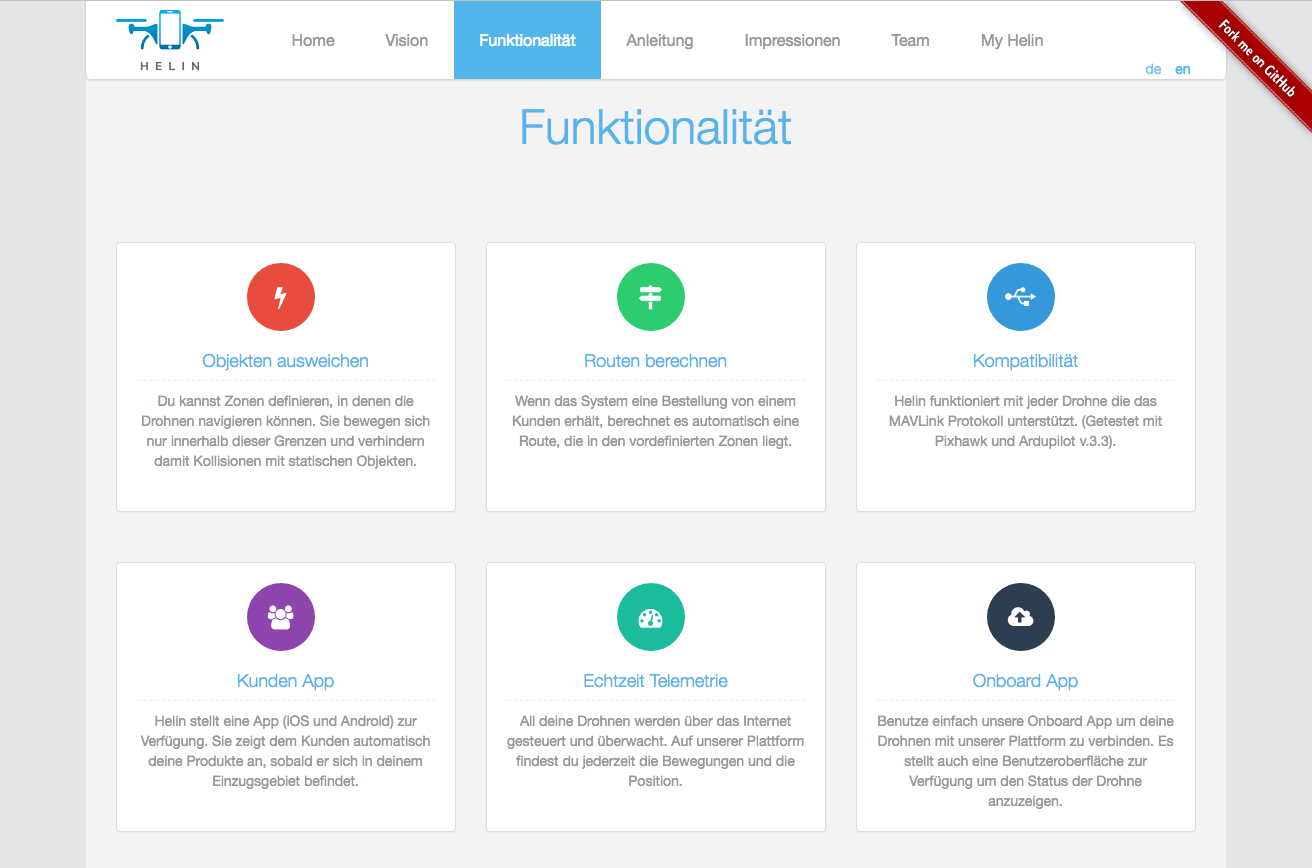
\includegraphics[width=1\textwidth] {images/website.png}
	\caption{Ausschnitt der Webseite \url{www.helin.ch}}
\end{figure}
\newpage

Ausserdem wurde die Plattform auf \url{my.helin.ch} freigeschaltet und kann frei genutzt werden.

\begin{figure}[H]
	\centering
	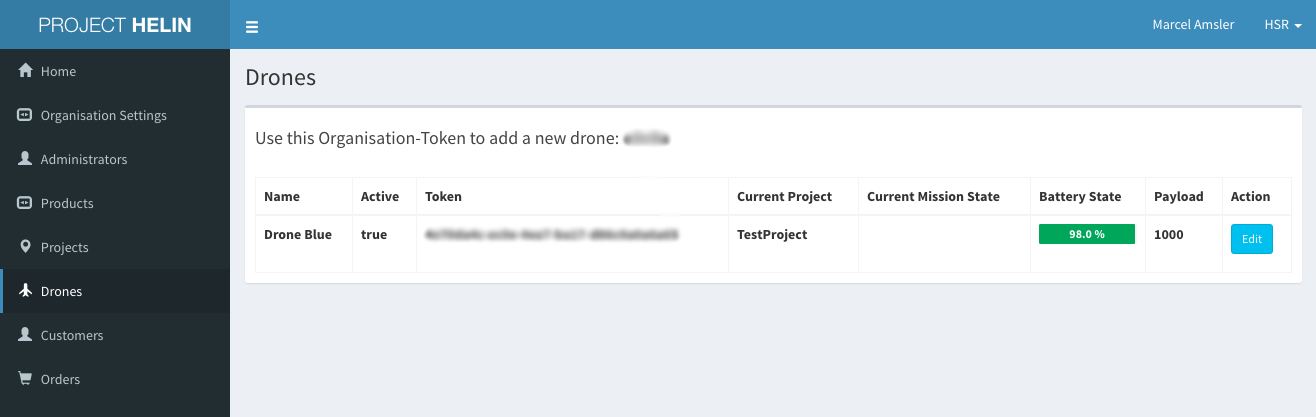
\includegraphics[width=1.0\textwidth] {images/myhelin.png}
	\caption{Drohnenliste von MyHelin}
\end{figure}

Die \Gls{Single-Page-Applications} für das Zeichnen von Zonen, das Testen eines Zonensetups und die Überwachung der Lieferungen stehen dann sofort zur Verfügung.

\begin{figure}[H]
	\centering
	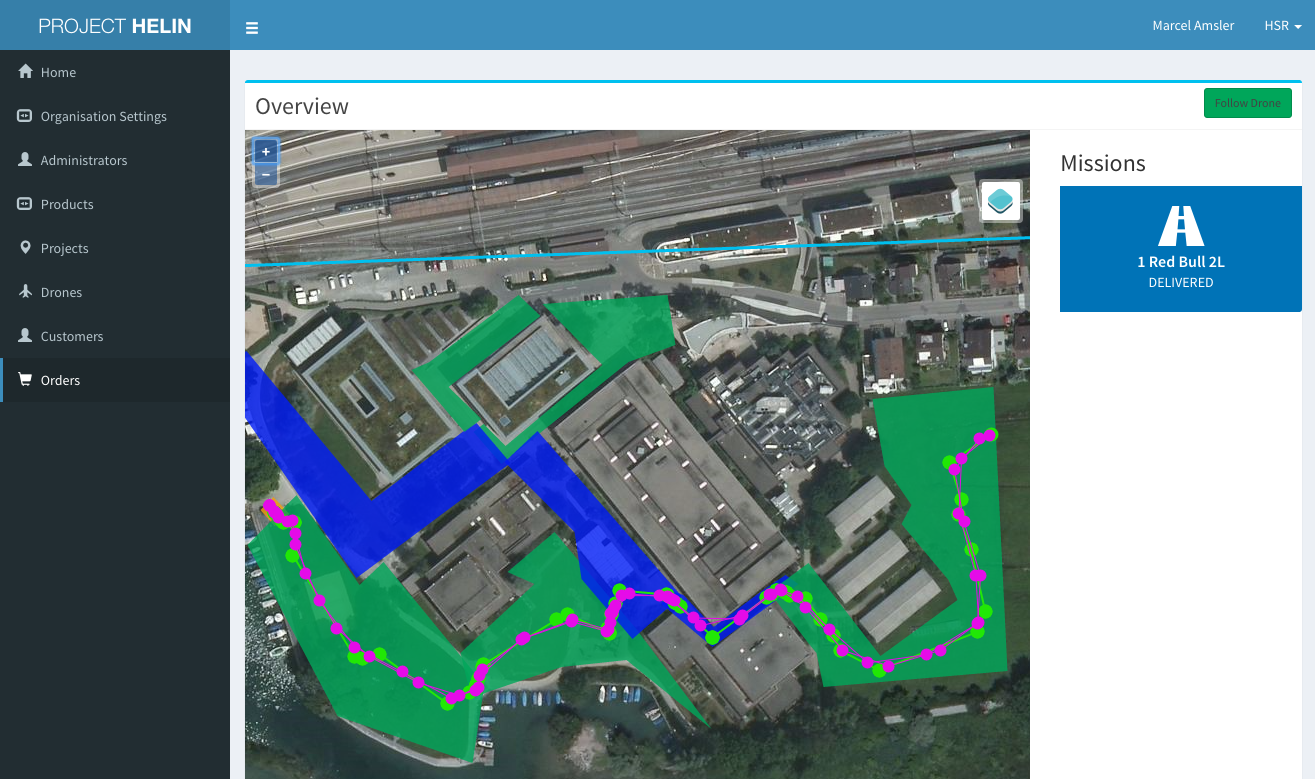
\includegraphics[width=1.0\textwidth] {images/map-ui.png}
	\caption{Kartenansicht bei der Verfolgung einer Drohne während der Mission}
\end{figure}

\newpage
Die verschiedenen Apps können aus dem jeweiligen App-Store oder direkt heruntergeladen werden.

\begin{figure}[H]
	\centering
	\begin{minipage}[b]{0.2\textwidth}
			\centering
		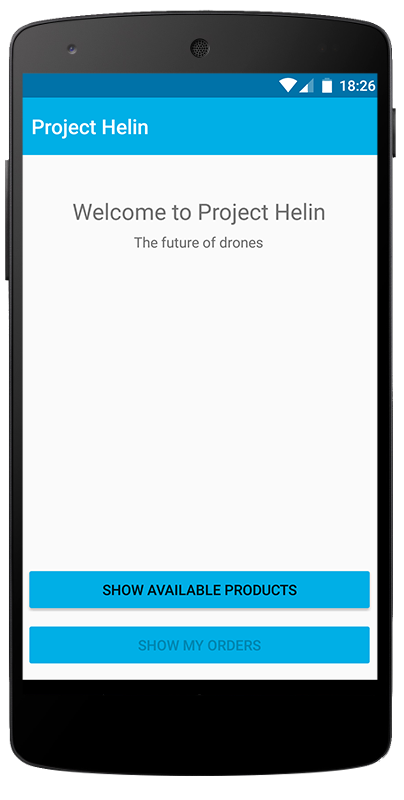
\includegraphics[width=\textwidth]{images/customer-app-android.png}
		\label{fig:customer-app-android}
	\end{minipage}
	\hfill
	\begin{minipage}[b]{0.2\textwidth}
		\centering
		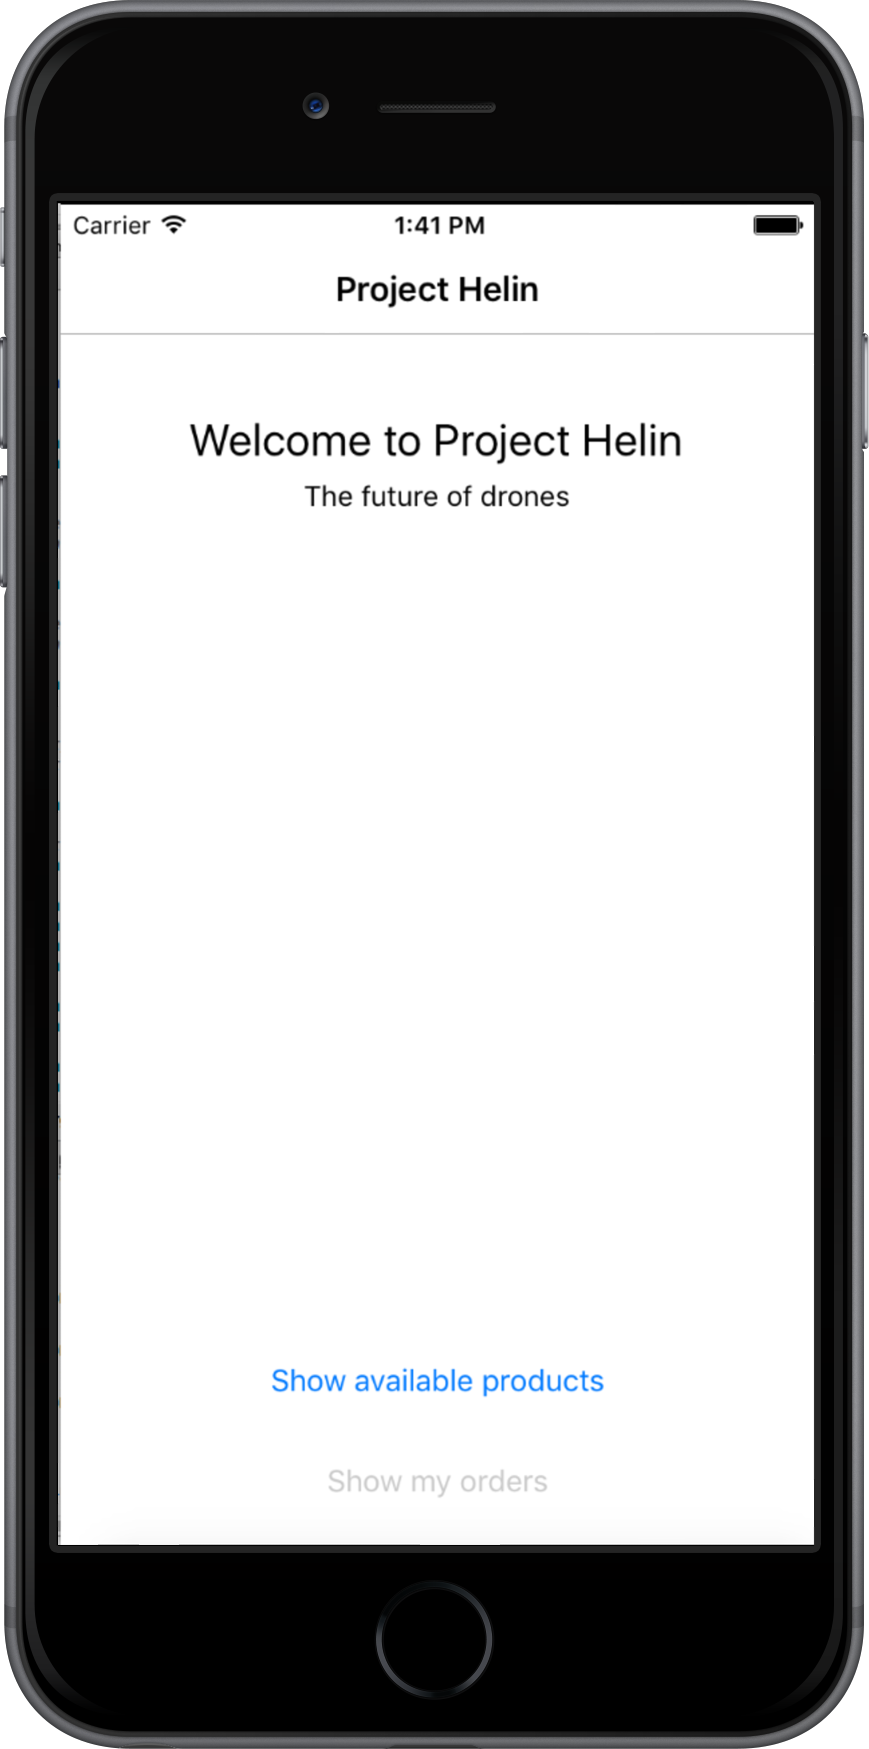
\includegraphics[width=\textwidth]{images/customer-app-ios.png}
		\label{fig:customer-app-ios}
	\end{minipage}
	\hfill
	\begin{minipage}[b]{0.2\textwidth}
			\centering
		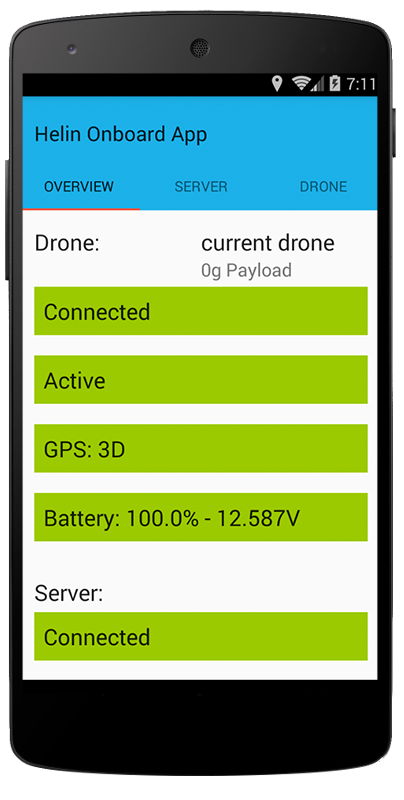
\includegraphics[width=\textwidth]{images/onboard-app.png}
		\label{fig:onboard-app-android}
	\end{minipage}
\end{figure}


Die Drohne zusammen mit dem Onboard-App konnte auf einen Stand gebracht werden in dem sie mehrere Lieferungen hintereinander ohne Schwierigkeiten ausführen kann.

\begin{figure}[H]
	\centering
	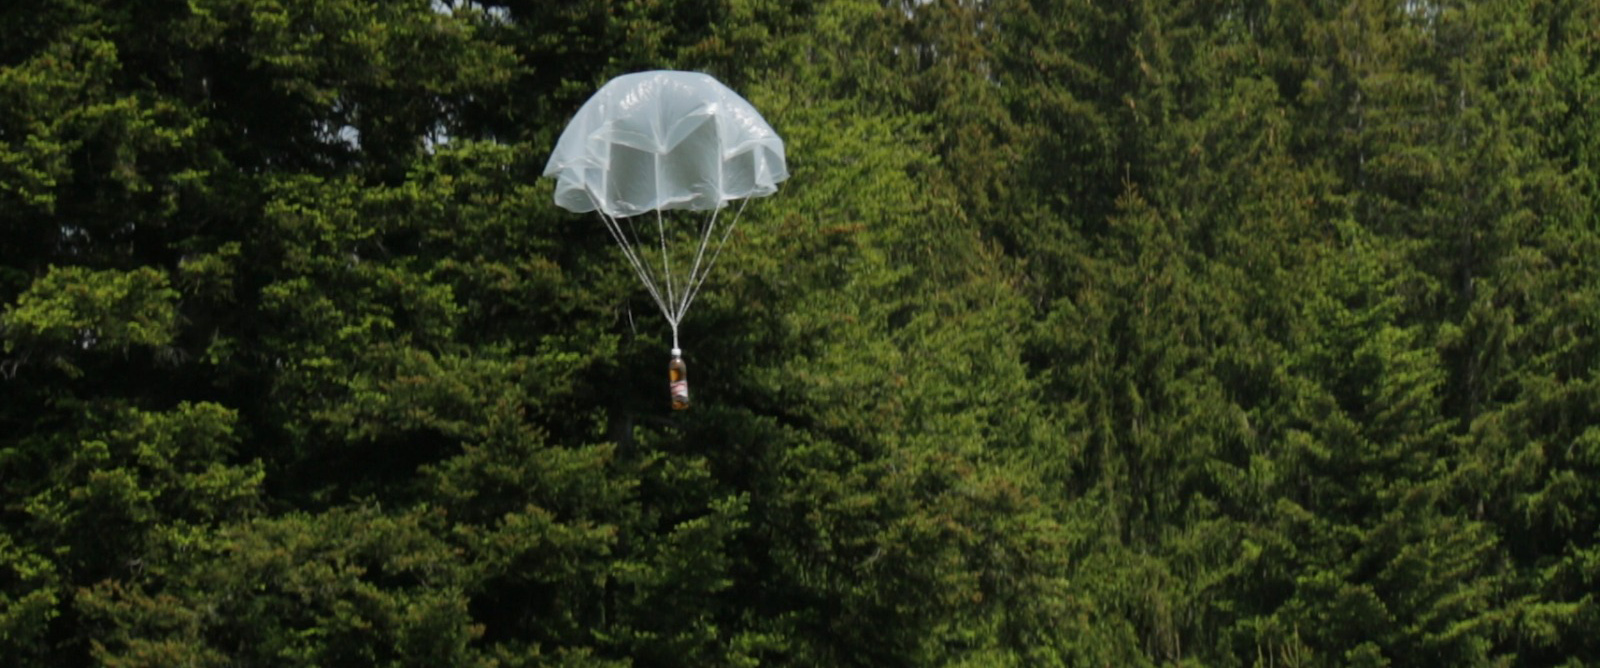
\includegraphics[width=1.0\textwidth] {images/parachute-test.jpeg}
	\caption{Diverse erfolgreiche Tests mit dem autonomen Abwurf der Ladung}
\end{figure}

\begin{figure}[H]
	\centering
	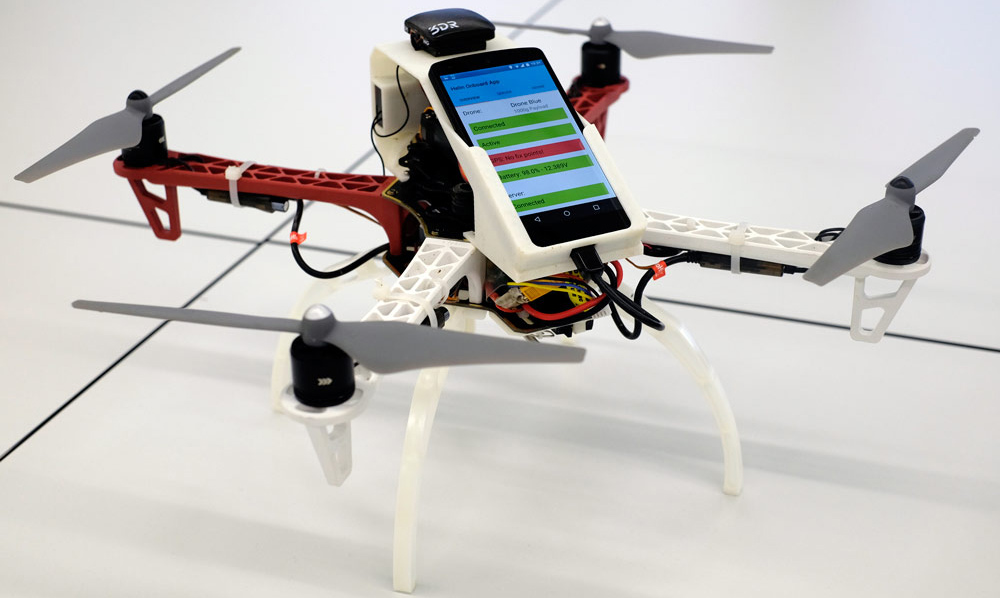
\includegraphics[width=1.0\textwidth] {images/drone.jpg}
	\caption{Drohne mit Onboard-App in der finalen Ausbaustufe}
\end{figure}



\subsection{Zusammenfassung der Ergebnisse}

Während dieser Arbeit hat das Team eine Plattform konzipiert und entwickelt, die es jedem Anbieter ermöglicht einen autonomen Drohnen-Lieferservice für ein von ihm definiertes Gebiet aufzubauen. Die Plattform wurde auf einem Server als Software as a Service zur Verfügung gestellt. Ausserdem wurde der gesamte Code des Projekts auf Github veröffentlicht und steht unter einer \Gls{MIT-Lizenz} als Open-Source-Software zur Verfügung. Die Tests mit den zwei eigens aufgebauten Drohnen zeigen, dass das System als ganzes funktioniert. \\

Folgende Ergebnisse sind besonders hervozuheben:

\begin{itemize}
	\item Webseite für Administratoren zur Verwaltung von Organisationen, Drohnen, Produkten und Bestellungen
	\item Cross-Plattform Bestell-App (iOS, Android) für Kunden
	\item Android App zur Steuerung der Drohne über das Internet
	\item Verfolgung der Drohnen-Telemetrie während, vor und nach der Lieferung einer Bestellung
	\item Automatisierte dynamische Routenberechnung über vordefinierte Flugzonen abhängig von der Position des Kunden
	\item Automatisierte Verteilung von Lieferaufträgen an die Drohnen
	\item Getestete Vorlage für den Aufbau einer Lieferdrohne
	\item Vorgefertigte 3D-Modelle für den 3D-Druck der Smartphone-Halterung und der Abwurfvorrichtung
\end{itemize}


\section{Ausblick}

Die entwickelte Plattform zeigt erst einen Bruchteil der Möglichkeiten, die in Zukunft von autonomen Drohnen übernommen werden können. Beispielsweise können Videoaufnahmen, Infrastruktur-Überwachung oder Katastrophenhilfe als Angebote integriert werden. 

\subsection{Empfohlene Weiterentwicklungen}

Während des Projekts sind weitere Ideen entstanden, die aber grössere Änderungen benötigen oder getestet werden müssen. Sie müssen für einen produktiven Einsatz aber nicht zwingend umgesetzt werden.

\subsubsection{Plattform}

\begin{itemize}
	\item Services hinzufügen (Drone-Selfie, Follow-Me Video, Geographische Vermessung)
	\item Aktion am Zielort wählbar oder vom Produkt abhängig machen
	\item Test ob es auch mit Radio-Telemetry am Onboard-App funktioniert
	\item Flight-Controller ohne MAVLink auch unterstützen (z.B. DJI-Onboard-SDK \cite{dji-sdk})
\end{itemize}

\subsubsection{Drohnen Hardware} 
\begin{itemize}
	\item Testen in Kombination mit Obstacle Avoidance (z.B. Intel RealSense\cite{realsense} Hardware)
		\item Tests mit anderen Arten von Drohnen (siehe Abschnitt \ref{sec:drone-alternatives})
	\item Smartphone ersetzen durch Embedded-System (siehe Alternativen im Abschnitt \ref{sec:communication-architecture}) 

	\item Automatisches Beladungssystem für Drohnen
	\item Automatisches Batterieaustauschsystem für Drohnen
\end{itemize}  



\subsection{Known-Issues}

Alle bekannten kleineren Probleme und zusätzlichen Features, die vor einem Produktiven Einsatz des Systems umgesetzt werden sollten, werden im Server-Github-Repository als Issues erfasst. Dies ermöglicht es auch anderen Entwicklern an dem Projekt weiterzuarbeiten und dessen Limitierungen zu kennen.


\section{Schlussfolgerung}

Während dieser Arbeit haben wir aus unserer Vision ein Produkt entwickelt und fertiggestellt. Damit konnten wir beweisen, dass man mit verfügbaren Technologien Liefersysteme mit autonomen Drohnen schon heute realisieren kann. Die entstandene Plattform kann nun zu Testzwecken von allen Interessierten genutzt und weiterentwickelt werden.\\

Die erarbeiteten funktionalen- und nicht-funktionalen Anforderungen konnten alle erfüllt und teilweise übertroffen werden, trotz der vielfältigen und teilweise interdisziplinären Aufgaben, die dieser Arbeit innewohnten. \\

Unserer Meinung nach ist unsere Plattform ein Beispiel für die Drohnen-Projekte der Zukunft. Vorallem im Bezug auf die Verwendung einer zentralen Instanz, zur Steuerung und Überwachung einer Drohnenflotte. Dadurch gewinnen viele Projekte wie das Überwachen von Haien \cite{shark}, die Lieferung von Defibrillatoren \cite{defibrillator-drone} oder das Finden von Überlebenden in einem Katastrophengebiet \cite{catastrophic-drone}, deutlich an praktischer Relevanz und können Flächendeckend eingesetzt werden. Wir hoffen, dass die entwickelte Plattform als Anstoss für die Stakeholder in dieser Branche dienen kann und sich die Technologien und Gesetzeslagen insoweit verbessern, dass Dienstleistungen von autonomen Drohnen bald für eine grössere Anzahl von Kunden zur Verfügung stehen werden.





